\documentclass[10pt,aspectratio=169]{beamer}

% ----------------------------------------------------------------------
% Blue Beamer theme
% ----------------------------------------------------------------------
\usetheme{Madrid}
\usecolortheme{default}
\definecolor{dauphineblue}{RGB}{0,81,186}
\setbeamercolor{structure}{fg=dauphineblue}
\setbeamercolor{palette primary}{bg=dauphineblue,fg=white}
\setbeamercolor{palette secondary}{bg=dauphineblue!80,fg=white}
\setbeamercolor{palette tertiary}{bg=dauphineblue!60,fg=white}
\setbeamercolor{frametitle}{bg=dauphineblue,fg=white}
\setbeamertemplate{navigation symbols}{}
\setbeamertemplate{caption}[numbered]

\usepackage[utf8]{inputenc}
\usepackage[T1]{fontenc}
\usepackage{lmodern}
\usepackage{amsmath}
\usepackage{graphicx}
\usepackage{booktabs}
\usepackage{tikz}
\usetikzlibrary{arrows.meta,positioning}

% Slightly smaller body text, following the "reduce by 20%" rule.
\setbeamerfont{normal text}{size=\small}
\AtBeginDocument{\small}

% Tighten the gap between the two columns and keep the block centered, so the
% text and the figure do not drift to the far edges of the slide.
\setlength{\columnsep}{1.2em}

% ----------------------------------------------------------------------
\title[Rubik's Cube with A*]{Solving the Rubik's Cube with A*}
\subtitle{Artificial Intelligence and Reasoning, Lab 1}
\author[CHEBBAH, BETRAOUI, SALL]{Mathias CHEBBAH \and Lamine BETRAOUI \and Bouna SALL}
\institute[Dauphine]{Universite Paris Dauphine, PSL \\ Master 1 MIAGE}
\date{June 2026}

\begin{document}

% ======================================================================
% COVER (not counted in the 9 slides)
% ======================================================================
\begin{frame}[plain]
  \titlepage
\end{frame}

% ======================================================================
% SLIDE 1
% ======================================================================
\begin{frame}{The problem}
  \begin{columns}[c,onlytextwidth]
    \hspace*{0.05\textwidth}
    \begin{column}{0.5\textwidth}
      \begin{itemize}
        \item A Rubik's Cube has six faces of nine stickers.
        \item Each face can turn, which mixes the colors.
        \item The cube is solved when each face is one color.
        \item It has about $4.3 \times 10^{19}$ configurations.
      \end{itemize}
      \vspace{0.25cm}
      \textbf{Our goal:} write the solve button. \\
      Find a list of moves back to the solved cube. \\
      We use search, as seen in Lecture 2.
    \end{column}
    \begin{column}{0.36\textwidth}
      \centering
      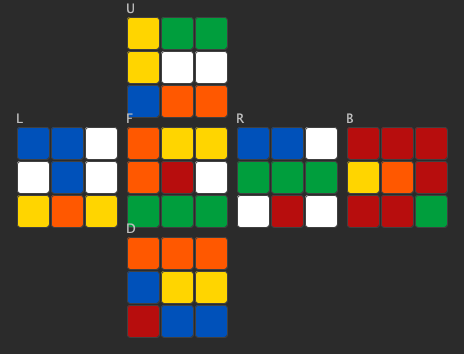
\includegraphics[width=\linewidth]{../report/figures/cube_scrambled.png} \\
      \vspace{0.15cm}
      {\tiny A scrambled cube, drawn as a net.}
    \end{column}
  \end{columns}
\end{frame}

% ======================================================================
% SLIDE 2
% ======================================================================
\begin{frame}{The cube as a search problem}
  \begin{columns}[T,onlytextwidth]
    \hspace*{0.05\textwidth}
    \begin{column}{0.5\textwidth}
      We use the five components of Lecture 2.
      \vspace{0.15cm}
      \begin{itemize}
        \item \textbf{State:} a cube configuration.
        \item \textbf{Actions:} the twelve quarter turns.
        \item \textbf{Transition:} a turn permutes the stickers.
        \item \textbf{Goal test:} every face is uniform.
        \item \textbf{Cost:} each move costs one.
      \end{itemize}
      \vspace{0.15cm}
      The shortest move list is the optimal solution. \\
      The branching factor is twelve, so the tree is $O(12^d)$. \\
      A blind search cannot go deep. We need a heuristic.
    \end{column}
    \begin{column}{0.34\textwidth}
      \centering
      \vspace{0.6cm}
      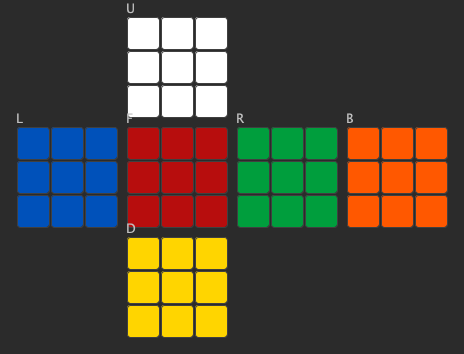
\includegraphics[width=\linewidth]{../report/figures/cube_solved.png} \\
      \vspace{0.1cm}
      {\footnotesize The goal state: every face uniform.}
    \end{column}
  \end{columns}
\end{frame}

% ======================================================================
% SLIDE 3
% ======================================================================
\begin{frame}{The classes}
  \begin{columns}[T,onlytextwidth]
    \hspace*{0.05\textwidth}
    \begin{column}{0.5\textwidth}
      We followed the statement closely, in Java.
      \vspace{0.15cm}
      \begin{itemize}
        \item \textbf{Cube:} faces, the twelve turns, isSolved.
        \item \textbf{State:} a node, with $g$, $h$ and expand.
        \item \textbf{Astar:} the solve method.
        \item \textbf{StateSet:} the explored set.
        \item \textbf{PriorityQueueState:} the frontier.
        \item \textbf{Heuristic:} the interface and two versions.
      \end{itemize}
      \vspace{0.15cm}
      The turns come from a real 3D model of the cube. \\
      We built each class test first, with twenty four tests.
    \end{column}
    \begin{column}{0.34\textwidth}
      \centering
      \vspace{0.5cm}
      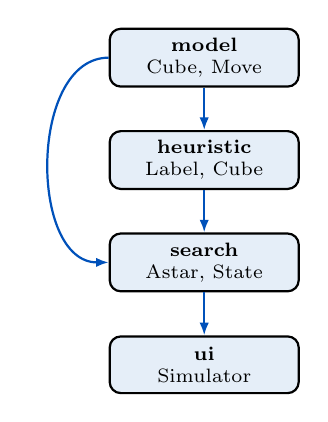
\begin{tikzpicture}[font=\scriptsize,
        box/.style={draw,thick,rounded corners,fill=dauphineblue!10,
                    minimum width=2.4cm,minimum height=0.72cm,align=center},
        arr/.style={-{Latex[length=1.6mm]},thick,dauphineblue}]
        \node[box] (m) at (0,3.0) {\textbf{model}\\ Cube, Move};
        \node[box] (h) at (0,1.7) {\textbf{heuristic}\\ Label, Cube};
        \node[box] (s) at (0,0.4) {\textbf{search}\\ Astar, State};
        \node[box] (u) at (0,-0.9) {\textbf{ui}\\ Simulator};
        \draw[arr] (m) -- (h);
        \draw[arr] (h) -- (s);
        \draw[arr] (m.west) to[out=180,in=180] (s.west);
        \draw[arr] (s) -- (u);
      \end{tikzpicture} \\
      \vspace{0.1cm}
      {\footnotesize The four packages.}
    \end{column}
  \end{columns}
\end{frame}

% ======================================================================
% SLIDE 4
% ======================================================================
\begin{frame}{The A* algorithm}
  \begin{columns}[T,onlytextwidth]
    \hspace*{0.05\textwidth}
    \begin{column}{0.5\textwidth}
      A* expands the node with the smallest value
      \[
        f(n) = g(n) + h(n).
      \]
      \begin{itemize}
        \item $g(n)$ is the cost from the start.
        \item $h(n)$ estimates the cost to the goal.
        \item An admissible $h$ never overestimates.
        \item With an admissible $h$, A* is optimal.
        \item With $h = 0$, A* is a uniform cost search.
      \end{itemize}
      \vspace{0.1cm}
      We rebuild the plan by walking the parent chain.
    \end{column}
    \begin{column}{0.34\textwidth}
      \centering
      \vspace{0.7cm}
      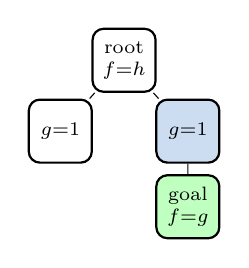
\begin{tikzpicture}[scale=0.6,
        every node/.style={draw,thick,rounded corners,align=center,
                           minimum size=8mm,font=\scriptsize}]
        \node (r) at (0,2.2) {root\\$f{=}h$};
        \node (a) at (-1.35,0.7) {$g{=}1$};
        \node[fill=dauphineblue!20] (b) at (1.35,0.7) {$g{=}1$};
        \node[fill=green!25] (g) at (1.35,-0.9) {goal\\$f{=}g$};
        \draw (r)--(a); \draw (r)--(b); \draw (b)--(g);
      \end{tikzpicture} \\
      \vspace{0.15cm}
      {\footnotesize The leaf with the smallest $f$ is expanded first.}
    \end{column}
  \end{columns}
\end{frame}

% ======================================================================
% SLIDE 5
% ======================================================================
\begin{frame}{Uniform cost search and A*}
  \begin{columns}[T,onlytextwidth]
    \hspace*{0.05\textwidth}
    \begin{column}{0.5\textwidth}
      \vspace{0.3cm}
      \begin{itemize}
        \item UCS orders the frontier by $g$ only.
        \item It is optimal but blind.
        \item A* adds the heuristic $h$.
        \item It looks toward the goal.
        \item So A* expands far fewer states.
        \item Both find the same optimal plan.
      \end{itemize}
    \end{column}
    \begin{column}{0.36\textwidth}
      \centering
      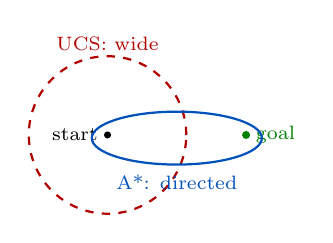
\begin{tikzpicture}[scale=0.8,font=\scriptsize]
        % start and goal
        \fill[black] (0,0) circle (1.6pt) node[left]{start};
        \fill[green!50!black] (2.2,0) circle (1.8pt) node[right]{goal};
        % UCS: wide circle around start
        \draw[red!70!black,thick,dashed] (0,0) circle (1.25);
        \node[red!70!black] at (0,1.45) {UCS: wide};
        % A*: narrow ellipse pointing to goal
        \draw[dauphineblue,thick,rotate around={0:(1.1,-0.05)}]
            (1.1,-0.05) ellipse (1.35 and 0.42);
        \node[dauphineblue] at (1.1,-0.75) {A*: directed};
      \end{tikzpicture} \\
      \vspace{0.2cm}
      {\footnotesize A* explores toward the goal, UCS in all directions.}
    \end{column}
  \end{columns}
\end{frame}

% ======================================================================
% SLIDE 6
% ======================================================================
\begin{frame}{Heuristic 1: the sticker relaxation}
  \begin{columns}[T,onlytextwidth]
    \hspace*{0.05\textwidth}
    \begin{column}{0.5\textwidth}
      A relaxation drops some rules of the problem. \\
      Here each sticker may move on its own.
      \vspace{0.15cm}
      \begin{itemize}
        \item Each sticker must reach its correct face.
        \item Distance is 0, 1 or 2 quarter turns.
        \item We sum over all 54 stickers.
        \item We divide by 12 stickers moved per turn.
      \end{itemize}
      \[
        h_{\text{label}} = \frac{1}{12}\sum_{s=1}^{54} d(s).
      \]
      After one turn, the sum is 12, so $h = 1$. \\
      This is admissible, so A* stays optimal.
    \end{column}
    \begin{column}{0.34\textwidth}
      \centering
      \vspace{0.8cm}
      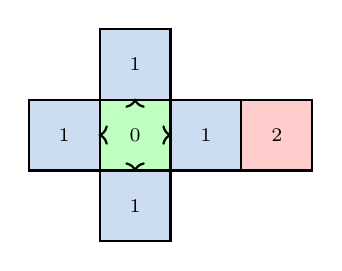
\begin{tikzpicture}[font=\scriptsize,scale=0.9,
        face/.style={draw,thick,minimum size=0.9cm}]
        \node[face,fill=green!25] (c) at (0,0) {0};
        \node[face,fill=dauphineblue!20] (u) at (0,1) {1};
        \node[face,fill=dauphineblue!20] (d) at (0,-1) {1};
        \node[face,fill=dauphineblue!20] (l) at (-1,0) {1};
        \node[face,fill=dauphineblue!20] (r) at (1,0) {1};
        \node[face,fill=red!20] (o) at (2,0) {2};
        \draw[->,thick] (u)--(c); \draw[->,thick] (d)--(c);
        \draw[->,thick] (l)--(c); \draw[->,thick] (r)--(c);
      \end{tikzpicture} \\
      \vspace{0.15cm}
      {\footnotesize Distance to the correct face: same 0, next 1, opposite 2.}
    \end{column}
  \end{columns}
\end{frame}

% ======================================================================
% SLIDE 7
% ======================================================================
\begin{frame}{Heuristic 2: the piece relaxation}
  \begin{columns}[T,onlytextwidth]
    \hspace*{0.05\textwidth}
    \begin{column}{0.5\textwidth}
      Here each piece may move on its own.
      \vspace{0.15cm}
      \begin{itemize}
        \item A piece is a corner or an edge.
        \item One turn moves four corners and four edges.
        \item We count the misplaced pieces.
        \item The centers are fixed, so we ignore them.
      \end{itemize}
      \[
        h_{\text{cube}} = \max\left(
        \left\lceil \tfrac{\text{misplaced corners}}{4} \right\rceil,
        \left\lceil \tfrac{\text{misplaced edges}}{4} \right\rceil
        \right).
      \]
      This is also admissible. The sticker one is stronger.
    \end{column}
    \begin{column}{0.34\textwidth}
      \centering
      \vspace{0.7cm}
      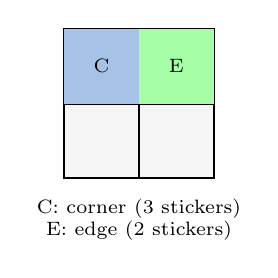
\begin{tikzpicture}[scale=0.95,font=\scriptsize]
        % a 2x2 grid representing a face, mark a corner and an edge
        \foreach \x in {0,1} \foreach \y in {0,1}
          \draw[thick,fill=gray!8] (\x,\y) rectangle ++(1,1);
        \fill[dauphineblue!35] (0,1) rectangle ++(1,1);
        \node at (0.5,1.5) {C};
        \fill[green!35] (1,1) rectangle ++(1,1);
        \node at (1.5,1.5) {E};
        \node[align=center] at (1,-0.55) {C: corner (3 stickers)\\ E: edge (2 stickers)};
      \end{tikzpicture}
    \end{column}
  \end{columns}
\end{frame}

% ======================================================================
% SLIDE 8
% ======================================================================
\begin{frame}{Results}
  \begin{columns}[c,onlytextwidth]
    \hspace*{0.05\textwidth}
    \begin{column}{0.5\textwidth}
      \begin{itemize}
        \item UCS blows up around depth seven.
        \item At depth six it expands about 500k states.
        \item Both heuristics scale much further.
        \item Plans stay optimal, same length.
        \item A* solves depth ten in about twelve seconds.
        \item Memory is the first limit, not time.
      \end{itemize}
    \end{column}
    \begin{column}{0.36\textwidth}
      \centering
      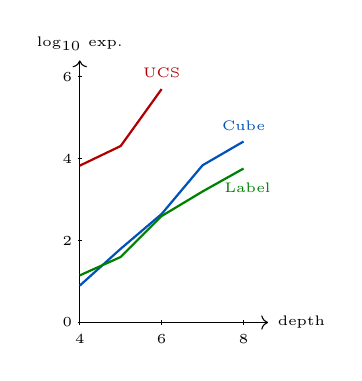
\begin{tikzpicture}[scale=0.52]
        \draw[->] (4,0) -- (8.6,0) node[right]{\tiny depth};
        \draw[->] (4,0) -- (4,6.4) node[above]{\tiny $\log_{10}$ exp.};
        \foreach \x in {4,6,8} \draw (\x,0.05)--(\x,-0.05) node[below]{\tiny \x};
        \foreach \y in {0,2,4,6} \draw (3.95,\y)--(4.05,\y) node[left]{\tiny \y};
        \draw[thick,red!70!black] (4,3.83)--(5,4.31)--(6,5.70);
        \node[red!70!black,font=\tiny] at (6,6.1) {UCS};
        \draw[thick,dauphineblue] (4,0.9)--(5,1.8)--(6,2.65)--(7,3.84)--(8,4.42);
        \node[dauphineblue,font=\tiny] at (8,4.8) {Cube};
        \draw[thick,green!50!black] (4,1.15)--(5,1.6)--(6,2.6)--(7,3.2)--(8,3.76);
        \node[green!50!black,font=\tiny] at (8.1,3.3) {Label};
      \end{tikzpicture} \\
      {\tiny Expanded states by depth, log scale.}
    \end{column}
  \end{columns}
\end{frame}

% ======================================================================
% SLIDE 9
% ======================================================================
\begin{frame}{Conclusion}
  \begin{columns}[T,onlytextwidth]
    \hspace*{0.05\textwidth}
    \begin{column}{0.5\textwidth}
      \vspace{0.3cm}
      \begin{itemize}
        \item We solved the cube with A*, as in the course.
        \item A* returns an optimal solution.
        \item A good heuristic gives huge savings.
        \item The heuristic changes the effort, not the answer.
        \item UCS fails from about seven moves.
        \item The main limit of A* is memory.
      \end{itemize}
    \end{column}
    \begin{column}{0.38\textwidth}
      \centering
      \vspace{0.4cm}
      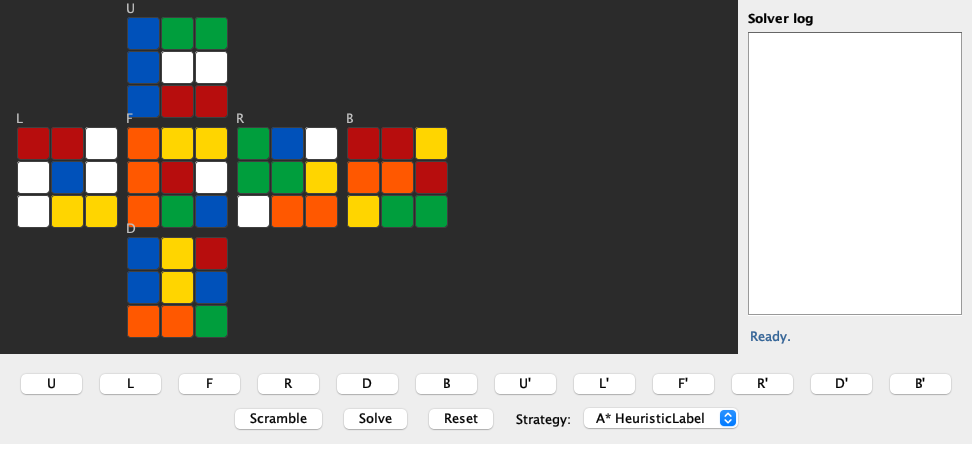
\includegraphics[width=\linewidth]{../report/figures/gui.png} \\
      \vspace{0.1cm}
      {\footnotesize Our simulator and its solve button.}
    \end{column}
  \end{columns}
  \vspace{0.3cm}
  \centering
  \textbf{Thank you for your attention.}
\end{frame}

\end{document}
